\chapter{神经网络概述}
\label{chap:neural-network-overview}

\BookChapterRef{chap:machine-learning-models}{第二卷“基础、理论和可信性”的“模型简介”章}
介绍过一种邮件分类方法：统计促销提示词和外部链接，再用加权和计算分类得分。这个方法能够学习各项特征的权重，却要由我们决定统计什么。如果判断还依赖词语之间的搭配、否定关系或句子上下文，仅仅调整已有特征的权重，未必能够表达这些关系。一个自然的问题是：能否把构造特征也交给学习算法，让模型根据任务需要改变自己的输入表示？

\term{人工神经网络}（artificial neural network, ANN）用相互连接的计算单元完成这种变换：一个单元组合已有数值，多个单元形成新的表示，再把这些表示交给后续计算。连接中的参数可以根据数据调整。这里的“神经”来自生物神经系统的启发；理解一个人工网络时，仍需具体说明它计算什么、信息怎样传递、哪些量参与学习。

本章围绕这几个问题建立共同框架。可学习表示说明网络怎样改变预测所依据的信息，生物启发说明这些计算抽象保留了什么、简化了什么。历史部分考察表示、学习和计算条件怎样共同发展，类型部分则用不同分类依据区分网络的结构假设。读者只需用到前文的特征、参数、损失函数和函数复合；各类网络的详细结构与训练推导将在后续章节展开。

\section{从人工特征到可学习的表示}
\label{sec:neural-learned-representations}

先把邮件分类器画成一个小网络，如图~\ref{fig:neural-minimal-mlp}所示。两个输入$x_1,x_2$仍是促销提示词和外部链接的统计量，但不再直接加权得到分类得分。中间三个单元各自读取这两个数，加权求和、加上偏置，再作非线性变换，得到$h_1,h_2,h_3$；输出单元将这三个数加权组合成得分$a$。中间这组单元称为\term{隐藏层}（hidden layer），因为它的数值由网络内部计算，而不是数据直接给出的输入或标签。这类具有一个或多个隐藏层、相邻层之间两两相连的逐层计算网络，称为\term{多层感知机}（multilayer perceptron, MLP）。图中的$2$-$3$-$1$分别表示输入、隐藏层和输出的单元数。

\begin{figure}[htbp]
  \centering
  % Two inputs, three hidden units, one score; biases are omitted.
\begin{tikzpicture}[x=1mm,y=1mm,font=\figurefont\footnotesize,text=NNInk]
  \foreach \i/\y in {1/8,2/-8}
    \node[nn input] (x\i) at (10,\y) {$x_{\i}$};
  \foreach \i/\y in {1/16,2/0,3/-16}
    \node[nn hidden] (h\i) at (53,\y) {$h_{\i}$};
  \node[nn output] (a) at (96,0) {$a$};
  \foreach \i in {1,2}
    \foreach \j in {1,2,3}
      \draw[nn link] (x\i)--(h\j);
  \foreach \j in {1,2,3}
    \draw[nn link] (h\j)--(a);
  \node[nn heading] at (10,29) {两个输入};
  \node[nn heading] at (53,29) {三个隐藏单元};
  \node[nn heading] at (96,29) {一个得分};
  \draw[nn flow] (22,22)--(40,22);
  \draw[nn flow,draw=NNOutput] (66,22)--(84,22);
  \node[nn annotation] at (53,-28) {前向计算：输入 $\to$ 隐藏数值 $\to$ 得分};
\end{tikzpicture}

  \caption{一个$2$-$3$-$1$多层感知机。两项输入先变成三个隐藏数值，再组合成一个分类得分。细线表示带权连接，箭头标出从左到右的计算方向；三个隐藏单元各作一次非线性变换，所有计算单元的偏置均省略。图只规定结构，权重尚未指定，也不要求某个隐藏单元预先代表某一种邮件特征。}
  \label{fig:neural-minimal-mlp}
\end{figure}
\FloatBarrier

围绕这个小网络，可以把学习中的三个问题分开。\term{表示能力}关心是否存在一组权重，使三个隐藏数值帮助输出端区分目标邮件；改变隐藏单元数，也会改变可选的计算。\term{优化}关心怎样根据训练邮件及其标签调整这些权重，让损失降低。\term{泛化}则关心训练后固定权重，面对未参与训练的新邮件时是否仍能作出可靠判断。画出网络还没有回答这三个问题，甚至原来的两项统计量也可能丢失判断所需的信息。下面从隐藏层怎样改变输入表示入手，再说明它与参数学习的联系。

\subsection{特征变换与函数复合}
\label{sec:neural-feature-composition}

线性得分是否够用，取决于它作用在哪种表示上。设输入为$\bm{x}\in\mathbb{R}^{d}$，预先确定的特征变换为$\bm{\phi}:\mathbb{R}^{d}\to\mathbb{R}^{m}$，线性得分可以写成
\begin{equation}
  f(\bm{x})=\bm{w}^{\top}\bm{\phi}(\bm{x})+b,
  \label{eq:neural-fixed-features}
\end{equation}
其中$\bm{w}\in\mathbb{R}^{m}$是权重，$b\in\mathbb{R}$是偏置。即使得分对$\bm{\phi}(\bm{x})$是线性的，只要特征变换包含平方、乘积等运算，它对原始输入也可以是非线性的。困难因而不只在分类器，还在于如何找到适合任务的$\bm{\phi}$。

神经网络把固定的特征变换换成带参数的变换。沿用前文的\term{表示学习}（representation learning）概念，这意味着模型从数据中学习供后续任务使用的信息形式，而不只学习最后的预测权重。将表示变换记为$\bm{r}_{\bm{\theta}}:\mathbb{R}^{d}\to\mathbb{R}^{m}$，输出映射记为$g_{\bm{\psi}}$，完整预测函数为
\begin{equation}
  f_{\bm{\theta},\bm{\psi}}(\bm{x})
  =g_{\bm{\psi}}\!\left(\bm{r}_{\bm{\theta}}(\bm{x})\right),
  \label{eq:neural-representation-readout}
\end{equation}
其中$\bm{\theta}\in\mathbb{R}^{p}$和$\bm{\psi}\in\mathbb{R}^{q}$分别收集表示部分与输出部分的参数，$p,q$是相应参数量。对于标量得分，$g_{\bm{\psi}}$可以仍是线性函数；它现在作用于模型自己构造的表示。

表示部分通常由若干次变换组成。以具有$L$个表示层的网络为例，令$\bm{h}^{(0)}=\bm{x}$，第$\ell$层的输出为$\bm{h}^{(\ell)}\in\mathbb{R}^{d_\ell}$，其中$d_0=d$。一种常见计算形式是
\begin{equation}
  \begin{aligned}
    \bm{h}^{(\ell)}
      &=\sigma_\ell\!\left(\bm{W}_\ell\bm{h}^{(\ell-1)}+\bm{b}_\ell\right),
      \qquad \ell=1,\ldots,L,\\
    \bm{r}_{\bm{\theta}}(\bm{x})&=\bm{h}^{(L)},
  \end{aligned}
  \label{eq:neural-layer-composition}
\end{equation}
其中$\bm{W}_\ell\in\mathbb{R}^{d_\ell\times d_{\ell-1}}$、$\bm{b}_\ell\in\mathbb{R}^{d_\ell}$分别是权重矩阵和偏置向量，$d_L=m$。本式中的$\sigma_\ell$逐坐标作用，称为\term{激活函数}（activation function），即在加权组合之后改变单元输出的函数。每个单元产生一个坐标；图~\ref{fig:neural-minimal-mlp}中的三个隐藏数值，就是这里$L=1$、$d_1=3$时的$\bm{h}^{(1)}$。

式\eqref{eq:neural-layer-composition}把函数复合落实为逐层计算：上一层的输出就是下一层的输入。若各层激活函数都是恒等函数，两层变换合起来为
\[
  \bm{W}_2(\bm{W}_1\bm{x}+\bm{b}_1)+\bm{b}_2
  =(\bm{W}_2\bm{W}_1)\bm{x}+\bm{W}_2\bm{b}_1+\bm{b}_2\text{。}
\]
结果仍是一次仿射变换，即线性变换加偏置。重复叠加这种层不会改变这一性质。非线性激活使不同输入范围能够产生不同响应，才让多层组合有机会表达原始坐标中的复杂关系。

\begin{example}[异或的表示变换]
  \label{ex:neural-xor-representation}
  考虑四个二值输入$\bm{x}=(x_1,x_2)^{\top}\in\{0,1\}^{2}$，目标在两个坐标不同时为$1$、相同时为$0$，这就是\term{异或}（exclusive OR, XOR）。设正类由$w_1x_1+w_2x_2+b>0$确定。若四个点都被正确分类，必须同时满足
  \[
    \begin{aligned}
      b&\leq0,& w_1+w_2+b&\leq0,\\
      w_1+b&>0,& w_2+b&>0\text{。}
    \end{aligned}
  \]
  第一行来自两个负例，第二行来自两个正例。两条正类约束相加得到$w_1+w_2+2b>0$，两条负类约束相加却得到同一表达式不大于$0$，所以这样的线性得分不存在。

  令$\rho(a)=\max\{0,a\}$，它保留非负值、把负值置零，称为\term{整流线性单元}（rectified linear unit, ReLU）的激活函数。构造两个隐藏单元
  \begin{equation}
    h_1=\rho(x_1-x_2),\qquad h_2=\rho(x_2-x_1),
    \label{eq:neural-xor-hidden}
  \end{equation}
  则四个输入的表示依次为
  \[
    \begin{aligned}
      (0,0)&\mapsto(0,0),& (1,1)&\mapsto(0,0),\\
      (1,0)&\mapsto(1,0),& (0,1)&\mapsto(0,1)\text{。}
    \end{aligned}
  \]
  在新表示中，用$h_1+h_2>1/2$判断正类就能全部分对。这组参数是为说明机制而手工构造的，并非一次训练的实验结果；它证明了隐藏表示可以解决原始坐标中的线性不可分问题。
\end{example}

图~\ref{fig:neural-xor-representation}给出这个例子的几何读法。变换没有修改标签，而是把两个负例送到同一个位置，把两个正例留在另外两个位置。输出层因此可以采用简单的分界。表示不必保留输入的每一项区别；在这个任务中，区分$(0,0)$和$(1,1)$并不是得到正确标签所必需的信息。

\begin{figure}[htbp]
  \centering
  % 原创教学示意。固定二值输入，按正文中两个 ReLU 单元的解析式变换。
\begin{tikzpicture}[x=1mm,y=1mm,font=\figurefont\footnotesize]
  \foreach \shift/\title/\xlabel/\ylabel in {
    0/原始表示/x_1/x_2,57/隐藏表示/h_1/h_2}{
    \begin{scope}[xshift=\shift mm]
      \node[font=\figurefont\bfseries\small] at (17,43) {\title};
      \fill[BookPaper] (0,0) rectangle (30,30);
      \draw[book arrow] (-3,0)--(35,0) node[right] {$\xlabel$};
      \draw[book arrow] (0,-3)--(0,35) node[above] {$\ylabel$};
      \node[below left] at (0,0) {$0$};
      \node[below] at (25,0) {$1$};
      \node[left] at (0,25) {$1$};
    \end{scope}
  }
  \fill[FigureInput] (0,0) circle (1.4);
  \fill[FigureInput] (25,25) circle (1.4);
  \fill[FigureLoss] (23.5,-1.5) rectangle (26.5,1.5);
  \fill[FigureLoss] (-1.5,23.5) rectangle (1.5,26.5);
  \draw[book arrow] (38,17)--(50,17);
  \begin{scope}[xshift=57mm]
    \draw[FigureModel,thick,dashed] (-2,14.5)--(14.5,-2);
    \fill[FigureInput] (0,0) circle (1.4);
    \fill[FigureLoss] (23.5,-1.5) rectangle (26.5,1.5);
    \fill[FigureLoss] (-1.5,23.5) rectangle (1.5,26.5);
    \node[align=center,text=BookMuted] at (18,26) {两正例分离};
    \node[align=center,text=BookMuted,anchor=north] at (15,-8) {两负例重合于原点};
  \end{scope}
  \node[anchor=north] at (14,-8) {线性不可分};
\end{tikzpicture}

  \caption{异或任务在变换前后的表示。圆点是标签为$0$的负例，方点是标签为$1$的正例。左侧两类点交错，无法用一条直线分开；右侧按式\eqref{eq:neural-xor-hidden}变换后，两个负例重合，虚线$h_1+h_2=1/2$将两类分开。坐标和变换均为教学构造。}
  \label{fig:neural-xor-representation}
\end{figure}

实际学习时，我们并不知道应该使用式\eqref{eq:neural-xor-hidden}中的权重。给定训练样本$S=((\bm{x}_i,y_i))_{i=1}^{n}$和损失函数$\ell$，可以把表示参数与输出参数放入同一个经验风险目标：
\begin{equation}
  \min_{\bm{\theta},\bm{\psi}}
  \frac{1}{n}\sum_{i=1}^{n}
  \ell\!\left(g_{\bm{\psi}}(\bm{r}_{\bm{\theta}}(\bm{x}_i)),y_i\right)\text{。}
  \label{eq:neural-joint-learning}
\end{equation}
两部分参数共同受最终任务的损失约束。这种\term{端到端学习}（end-to-end learning）把从输入到输出的一整条计算路径纳入同一学习目标。它仍需确定输入编码、网络结构和损失；对于不可微的操作，也需要另外设计参数更新方法。隐藏层能够表达有用特征、算法能够找到这些特征、得到的预测能用于新样本，是三个不同问题。

\subsection{分布式表示与层次表示}
\label{sec:neural-distributed-hierarchical}

一个隐藏向量有多个坐标，信息可以怎样放进这些坐标？如果每种对象只激活一个专属坐标，表示的区分主要由“哪一个坐标被激活”完成。\term{分布式表示}（distributed representation）采用另一种组织方式：一个对象由多个单元的活动共同表示，而同一个单元又可以参与多个对象的表示。这里的“分布式”指信息分布在若干坐标中，与把计算分配到多台机器是不同的概念。

一个简化例子是同时记录物体的颜色、形状和大小。若三个二值坐标分别表示“红色”“圆形”“较大”，那么$(1,1,0)$表示一个较小的红色圆形物体，$(1,0,0)$表示一个较小的红色非圆形物体。两个对象共享部分坐标，又在形状坐标上不同。三个二值坐标可以组成八种不同编码，说明共享属性能够通过组合区分对象；这只是编码数量的计算，不能据此推出模型用少量样本就一定能学会所有组合。

真实网络的坐标通常是连续数值，也未必逐一对应“颜色”这样的命名属性。表示中的信息可能需要若干坐标共同参与后续计算才能被读取。因而，某个单元响应某类输入，并不自动证明它只表示一个概念；分布式表示也可以是稀疏的，只要一个对象仍由若干可复用单元共同编码。这种对信息组织方式的理解，比把每个单元固定解释成一个符号更适合描述许多网络表示\scite{goodfellow2016}

分布式表示考察同一层内的信息怎样分配，\term{层次表示}（hierarchical representation）则考察不同层之间怎样组合信息：后层利用前层的表示继续构造新特征。以图像为例，一层可以响应局部明暗变化，后层再组合这些响应以识别纹理或形状。这里的“局部变化—组合模式”是理解层次结构的一条路径，不是所有网络必须遵循的固定语义顺序。层数越多，也不保证每一层的含义越抽象或越容易解释。

两种表示方式可以同时存在。一个层用多个单元共同表达某种形状，下一层再把这组活动与其他信息组合。图~\ref{fig:neural-representation-path}强调的正是这种计算关系：每层提供一组供后续使用的数值，最终预测又通过学习目标影响各层参数。表示是否有用，要结合后续任务判断；为了分类而压缩的区别，在重建输入时可能仍然需要保留。

\begin{figure}[htbp]
  \centering
  % 原创示意。实线为计算依赖，虚线为共同学习目标的约束关系。
\begin{tikzpicture}[x=1mm,y=1mm,font=\footnotesize]
  \node[book node,fill=FigureInput!12,minimum width=17mm] (x) at (9,0) {$\bm{x}$};
  \node[book node,fill=FigureModel!12,minimum width=20mm] (h1) at (36,0) {$\bm{h}^{(1)}$};
  \node[book node,fill=FigureModel!12,minimum width=20mm] (h2) at (65,0) {$\bm{h}^{(2)}$};
  \node[book node,fill=FigureOutput!12,minimum width=21mm] (out) at (95,0) {$g_{\bm{\psi}}(\bm{h}^{(2)})$};
  \draw[book arrow] (x)--(h1);
  \draw[book arrow] (h1)--(h2);
  \draw[book arrow] (h2)--(out);
  \node[below=2mm of x] {输入};
  \node[below=2mm of h1] {表示层};
  \node[below=2mm of h2] {表示层};
  \node[below=2mm of out] {输出};
  \node[book node,fill=FigureLoss!12,minimum width=38mm] (loss) at (66,-30) {训练目标：比较预测与标签};
  \draw[book arrow,dashed,draw=FigureLoss] (loss.north west)--(h1.south);
  \draw[book arrow,dashed,draw=FigureLoss] (loss.north)--(h2.south);
  \draw[book arrow,dashed,draw=FigureLoss] (loss.north east)--(out.south);
\end{tikzpicture}

  \caption{表示学习的一条计算路径。实线表示输入经过两层变换后交给输出映射，虚线表示同一个训练目标约束表示与输出两部分的参数。图只展示层间依赖，不要求隐藏坐标具有预先指定的语义，也不表示参数更新沿虚线完成一次普通前向计算。}
  \label{fig:neural-representation-path}
\end{figure}

\subsection{结构带来的归纳偏置}
\label{sec:neural-structural-bias}

允许学习表示，并没有规定所有输入都应怎样相互联系。若把图像中的每个像素与下一层所有单元相连，模型可以使用任意位置的组合，却没有直接体现相邻像素往往共同形成局部模式这一特点。网络结构可以预先限定哪些信息被组合、哪些计算被重复使用，从而影响学习时优先考虑的规律。

这种预先的限制或偏好称为\term{归纳偏置}（inductive bias）：面对有限数据，学习方法依据哪些假设把已经看到的关系推广到未见输入。偏置可以来自结构，也可以来自参数约束、损失和学习算法。这里聚焦结构，考察它怎样改变候选函数与信息传递路径。

\term{局部连接}（local connectivity）让一个单元只读取某个邻域的信息，例如图像中的一小块像素。\term{参数共享}（parameter sharing）让多个位置重复使用同一组参数，例如把同一个局部模式检测器移到图像各处。这两项设计分别规定“看哪些输入”和“在哪些位置使用同一种计算”。它们可以减少独立参数的数量，并使不同位置的数据共同参与共享参数的学习；具体效果仍取决于数据是否具有相应的局部性和重复规律。

对序列而言，结构还可以保留\term{隐状态}（hidden state），即在处理当前输入时保存一组由历史输入计算得到的数值。下一步继续读取这组数值，就能利用此前的信息。例如，看到“虽然”之后，后续判断可能需要继续保留尚未完成的转折关系。状态的存在提供了记忆通道，但状态维度、更新方式和学习过程仍会限制实际能够保留的信息。

结构假设匹配数据时，学习算法无需为每个位置或时间步单独发现同一种关系。假设不匹配时，同样的限制也可能排除需要的函数：只允许狭小邻域交互，可能难以直接比较相隔很远的对象；强制不同位置使用同一参数，可能忽略位置本身的特殊意义。网络设计需要在表达能力、样本利用与计算成本之间作出取舍。
\BookChapterRef{chap:deep-learning-theory}{第二卷“基础、理论和可信性”的“深度学习的可学习性”章}
已经说明，架构允许哪些函数与训练算法选出哪个函数分别影响学习结果，不能从结构名称直接得到泛化保证。

\section{生物神经网络}
\label{sec:neural-biological-inspiration}

人工网络为什么借用“神经元”“连接”和“学习”这些名称？理解它们的来源，需要同时看细胞怎样通信、系统怎样组织信息，以及经验怎样改变连接。本节从这三个方面介绍生物神经网络，再比较人工网络保留了哪些计算思想、哪些细节需要另外建模。

\subsection{神经元}
\label{sec:neural-biological-unit}

生物\term{神经元}（neuron）是接收和传递信号的细胞。许多神经元通过树突和胞体接收输入，\term{膜电位}（membrane potential），也就是细胞膜内外的电势差，随输入和细胞内部动态变化。在适当条件下，神经元产生称为\term{动作电位}（action potential）的短暂电信号，通常也称脉冲，并沿轴突影响其他细胞。神经元之间传递影响的连接部位称为\term{突触}（synapse），其传递效果可以随活动发生变化。这里概括的是典型脉冲神经元的部分机制，不覆盖所有细胞类型和信号传递方式。

图~\ref{fig:neural-biological-neuron}用一个神经元连接另外两个神经元的回路，把接收与传递信号的结构展开。树突从胞体向外分支，提供与其他细胞发生交互的部位；轴突则把信号传到末梢，末梢可以与其他细胞形成突触。支持神经元活动的\term{胶质细胞}（glial cell）参与维持细胞环境和形成髓鞘等过程。部分轴突外包有\term{髓鞘}（myelin sheath），即胶质细胞形成的多层膜结构，有助于加快传导。相邻髓鞘段之间的间隙称为\term{郎飞结}（node of Ranvier），动作电位在这些位置再生。在脑中，髓鞘由少突胶质细胞形成；神经元的形态各异，也并非所有轴突都有髓鞘\scite{purves2001}

\begin{figure*}[!t]
  \centering
  \resizebox{\linewidth}{!}{% 一幅完整的生成式解剖插画：神经元1的轴突分支影响神经元2和3。
% 全部标注、引导线与传递方向由 TikZ 排版；不重复拼接单细胞素材。
\begin{tikzpicture}[x=1mm,y=1mm,font=\kaishu\footnotesize,
  leader/.style={draw=BookMuted,line width=0.5pt},
  annotation/.style={fill=white,inner sep=0.7mm},
  transmission/.style={book arrow,draw=BookTeal,line width=1pt}]
  \node[anchor=south west,inner sep=0pt] at (0,0)
    {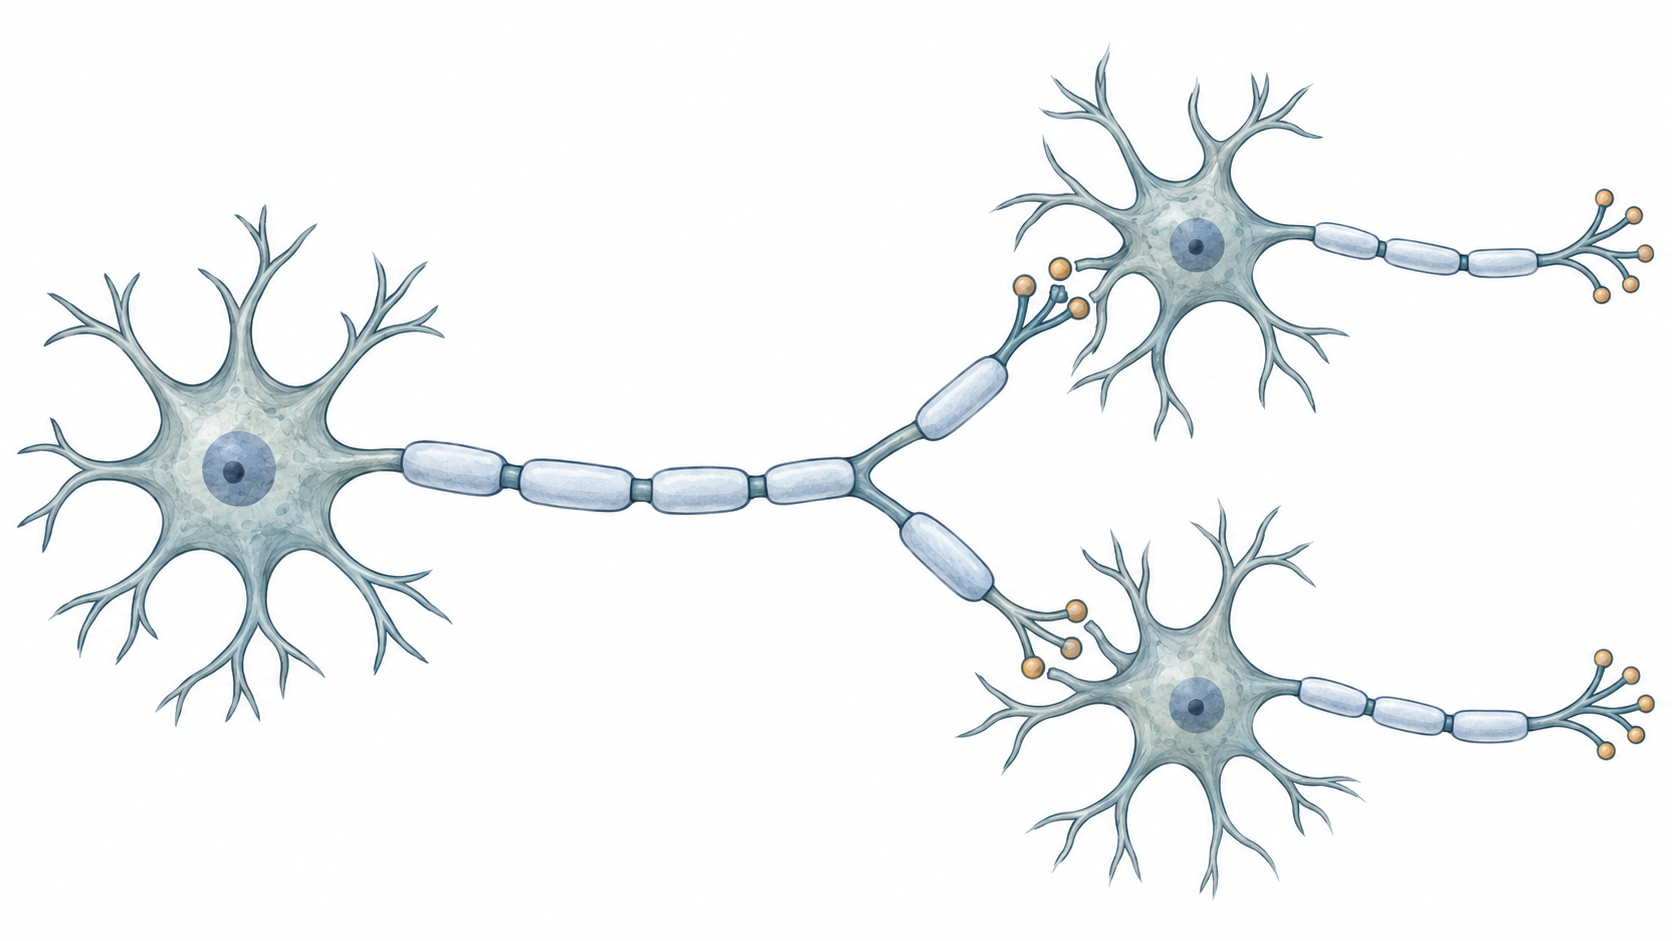
\includegraphics[width=168mm]{figures/neural-overview-neuron-divergence.png}};
  \node[annotation] at (25,86) {神经元1};
  \node[annotation] at (140,91) {神经元2};
  \node[annotation] at (142,6) {神经元3};
  \node[annotation] (dendrites) at (9,76) {树突};
  \draw[leader] (dendrites.south)--(9,70)--(11,64);
  \node[annotation] (soma) at (9,23) {胞体};
  \draw[leader] (soma.north)--(10,29)--(18,43);
  \node[annotation] (nucleus) at (35,21) {细胞核};
  \draw[leader] (nucleus.north)--(32,31)--(24,47);
  \node[annotation] (axon) at (41,64) {轴突};
  \draw[leader] (axon.south)--(41,57)--(37,48);
  \node[annotation] (myelin) at (59,65) {髓鞘};
  \draw[leader] (myelin.south)--(59,58)--(57,46);
  \node[annotation] (ranvier) at (67,26) {郎飞结};
  \draw[leader] (ranvier.north)--(67,34)--(64.4,45.3);
  \node[annotation] (branch) at (86,59) {轴突分支};
  \draw[leader] (branch.south)--(86,51)--(86,46);
  \node[annotation] (terminals) at (91,80) {轴突末梢};
  \draw[leader] (terminals.south)--(96,75)--(102.8,66);
  \node[annotation] (synapseone) at (110,53) {突触1};
  \draw[leader] (synapseone.north)--(110,60)--(107.1,67.5);
  \node[annotation] (synapsetwo) at (91,14) {突触2};
  \draw[leader] (synapsetwo.north)--(98,24)--(108.7,32.3);
  \draw[transmission] (43,53)--(77,53);
  \node[annotation,text=BookTeal] at (61,57) {信号传递};
  \draw[transmission] (87,51) to[out=35,in=215] (98,62);
  \draw[transmission] (87,40) to[out=-35,in=155] (99,33);
\end{tikzpicture}
}
  \caption{三个神经元在同一幅画面中通过突触相连。细线标出树突、胞体、细胞核、轴突、髓鞘、郎飞结与轴突末梢；青色箭头概括神经元1的轴突分成两支，分别经突触1和突触2影响神经元2和神经元3的方向，金黄色末梢表示突触前端。突触处的微小间隙只作概念提示。图展示一种多极、有髓鞘的神经元形态，各部分不按比例；真实神经元形态多样，部分轴突没有髓鞘，回路也可以包含反馈和更多连接。}
  \label{fig:neural-biological-neuron}
\end{figure*}

信号到达末梢后，怎样影响下一个细胞？在常见的\term{化学突触}（chemical synapse）中，动作电位促使末梢释放\term{神经递质}（neurotransmitter），即传递影响的化学信号分子。递质穿过两细胞之间的狭小间隙，与接收侧的受体作用，进而改变离子通道活动和膜电位。输入的作用可以是促进，也可以是抑制脉冲发放，具体取决于受体、通道与细胞状态。\term{电突触}（electrical synapse）则通过连接两细胞的通道直接传递电流。因此，图中的连接不能统一理解成把一个数值无延迟地送给下一个单元的导线\scite{purves2001}

接收到一次输入，并不意味着细胞必然发放一次脉冲。突触输入引起的膜电位变化会持续一段时间，再逐渐衰减；若其他输入在这段时间内到达，它们的影响就可能共同改变细胞的响应。来自多个连接的输入与同一连接在不同时间到达的输入，都可以参与这种整合，抑制性输入又可能降低发放的机会。在简化模型中，可以把较弱输入的影响近似相加，并用阈值描述何时发放；真实细胞的整合还取决于树突位置、膜上的通道和近期活动，未必只是一个静态加权和\scite{gerstner2014}

\Needspace{6\baselineskip}
脉冲的个数与发生时刻都可以参与信息表达。例如，同样发放3次脉冲，集中在短时间内与分散在较长时间内，对接收细胞可能产生不同影响；单个细胞的活动又需要放在其他细胞的共同活动中理解。许多典型动作电位持续约$1$至$2\,\mathrm{ms}$，这是细胞信号的时间尺度，不能直接当作大脑完成一个判断所需的时间。判断可能依赖多个回路中的持续活动与往返交互\scite{gerstner2014}

\FloatBarrier
\subsection{神经系统}
\label{sec:neural-biological-system}

单个细胞的接收和发放机制，还不能解释视觉、记忆或动作怎样形成。神经元连接成局部回路，多个回路再参与更大范围的神经系统。按解剖位置，人类神经系统通常分为脑与脊髓组成的\term{中枢神经系统}（central nervous system, CNS），以及联系中枢与身体其他部分的\term{外周神经系统}（peripheral nervous system, PNS）。感觉输入、内部活动和动作输出通过这些系统相互联系；下面主要考察人脑，尤其是与人工视觉模型联系较紧密的大脑皮层\scite{purves2001}

先看这种启发来自多大规模的系统。Azevedo等在2009年分析了4个年龄为50至71岁的成年男性脑样本，估计神经元数量的样本均值约为$861$亿，样本标准差约为$81$亿。这是常用的“人脑约有860亿个神经元”说法的一项主要依据。研究通过细胞核计数与神经元标记估算数量；这个结果应当用于理解规模，不能当作每个人都有同样数量的精确常数。同一研究中，大脑皮层约有$163$亿个神经元，小脑约有$690$亿个，分别约占总数的$19\%$和$80\%$。神经元数量在不同结构间很不均匀，数量最多的结构也不能仅凭这一点被认定为负责所有最复杂的认知任务\scite{azevedo2009}

这些细胞并非排成一组统一的层。脑内既有形成局部回路的连接，也有联系不同区域的长距离通路；大脑皮层、小脑和脑干等结构具有不同的细胞组织与连接方式。神经元与胶质细胞共同构成脑组织，后者还参与代谢支持等过程。因而，理解脑的架构，需要同时考察细胞类型、局部回路与区域间通信，不能只数计算单元\scite{purves2001}

脑的计算能力需要从这些网络的活动来理解。大量细胞可以同时接收输入和改变状态，计算分散在许多局部回路中；反馈连接又使当前响应依赖过去的活动。即使没有新的外部任务，脑内仍有持续的活动。并行性、内部状态与信号往返让脑能够处理随时间变化的感觉和行为信息，但这些特点本身不能给出某项任务的准确率，也不能由细胞数量推出每秒完成多少次通用算术运算。

维持这种活动还需要能量。成人脑的质量约占体重的$2\%$，却消耗全身约$20\%$的氧和相应代谢能量\scite{raichle2002}描述成人脑时，约$20\,\mathrm{W}$这一量级常用于表示葡萄糖供能对应的代谢功率；它包含通信与维持细胞功能等支出，各过程如何分摊能量还依赖具体的估算模型\scite{levy2021}这说明信息传递和维持活动也是计算系统的成本。若要与人工系统比较效率，需要固定任务、准确率、响应时间和能耗范围；把一次突触事件直接算作一次浮点运算，会忽略两者操作内容和精度的差异，得不到统一的“大脑算力”。

\FloatBarrier
这些局部回路和长距离连接在皮层中怎样组织？\term{大脑皮层}（cerebral cortex）是覆盖大脑半球表面的薄层组织，折叠形成沟和回。皮层属于\term{灰质}（gray matter），其中集中着细胞体、树突、突触与局部轴突；皮层下的\term{白质}（white matter）以轴突束为主要组成，为区域间通信提供通路。两种名称概括组织组成，并不是把脑机械分成“只计算”和“只传输”的两部分\scite{purves2001}

人脑大部分皮层属于\term{新皮层}（neocortex），按细胞密度、形态和连接等特征，通常从表面向内分成I至VI六个解剖层。不同层接收与发出的连接有所不同，层内存在横向联系，层间又有跨层联系。这里的“六层”是同一片皮层厚度方向上的组织分层；V1、V2等脑区各自包含自己的层内和层间回路，不能把这六层理解成人工网络连续执行的六个计算步骤\scite{purves2001}

层内与层间回路还与其他区域相连。以视觉为例，可以观察局部输入怎样经过多个区域，形成识别和行动所需的信息。\term{中央沟}（central sulcus）是区分额叶与顶叶的主要解剖标志，本身不是视觉计算阶段。图~\ref{fig:neural-visual-pathways}借助中央沟和各叶的位置定位视觉区，箭头表示主要传递方向。

视觉处理从眼中的\term{视网膜}（retina）开始，光在这里转化为神经信号，并经过局部回路处理。一条主要通路把视网膜神经节细胞的输出经丘脑的\term{外侧膝状体}（lateral geniculate nucleus, LGN）送到\term{初级视觉皮层}（primary visual cortex, V1）。V1主要位于枕叶内侧的距状沟周围，单从脑的外侧看不到它的大部分。V1之后的信号经V2等区域继续传递，逐渐进入分布在枕叶、颞叶与顶叶的多个视觉区域。这里描述的是主通路，视觉信号也参与眼动和反射等其他通路\scite{purves2001}

\begin{figure*}[!t]
  \centering
  \resizebox{\linewidth}{!}{% 自然解剖插画仅提供脑形态；全部区域定位与通路由 TikZ 精确叠加。
% 点位为教学投影而非实测区域边界；V1 内侧位置由右侧视图说明。
% 位置：Wandell et al. (2007), doi:10.1016/j.neuron.2007.10.012。
% 通路：Purves et al. (2001), Neuroscience；Goodale & Milner (1992)。
\begin{tikzpicture}[x=1mm,y=1mm,font=\figurefont\footnotesize,
  area/.style={circle,minimum size=2.5mm,inner sep=0pt,draw=BookInk,fill=white},
  annotation/.style={fill=white,inner sep=0.7mm},
  ventral/.style={book arrow,draw=BookAmber,line width=1.7pt,
    preaction={draw=white,line width=3.5pt}},
  dorsal/.style={book arrow,draw=BookBlue,line width=1.7pt,dashed,
    preaction={draw=white,line width=3.5pt}},
  leader/.style={draw=BookMuted,line width=0.5pt}]
  \node[anchor=south west,inner sep=0pt] at (0,0)
    {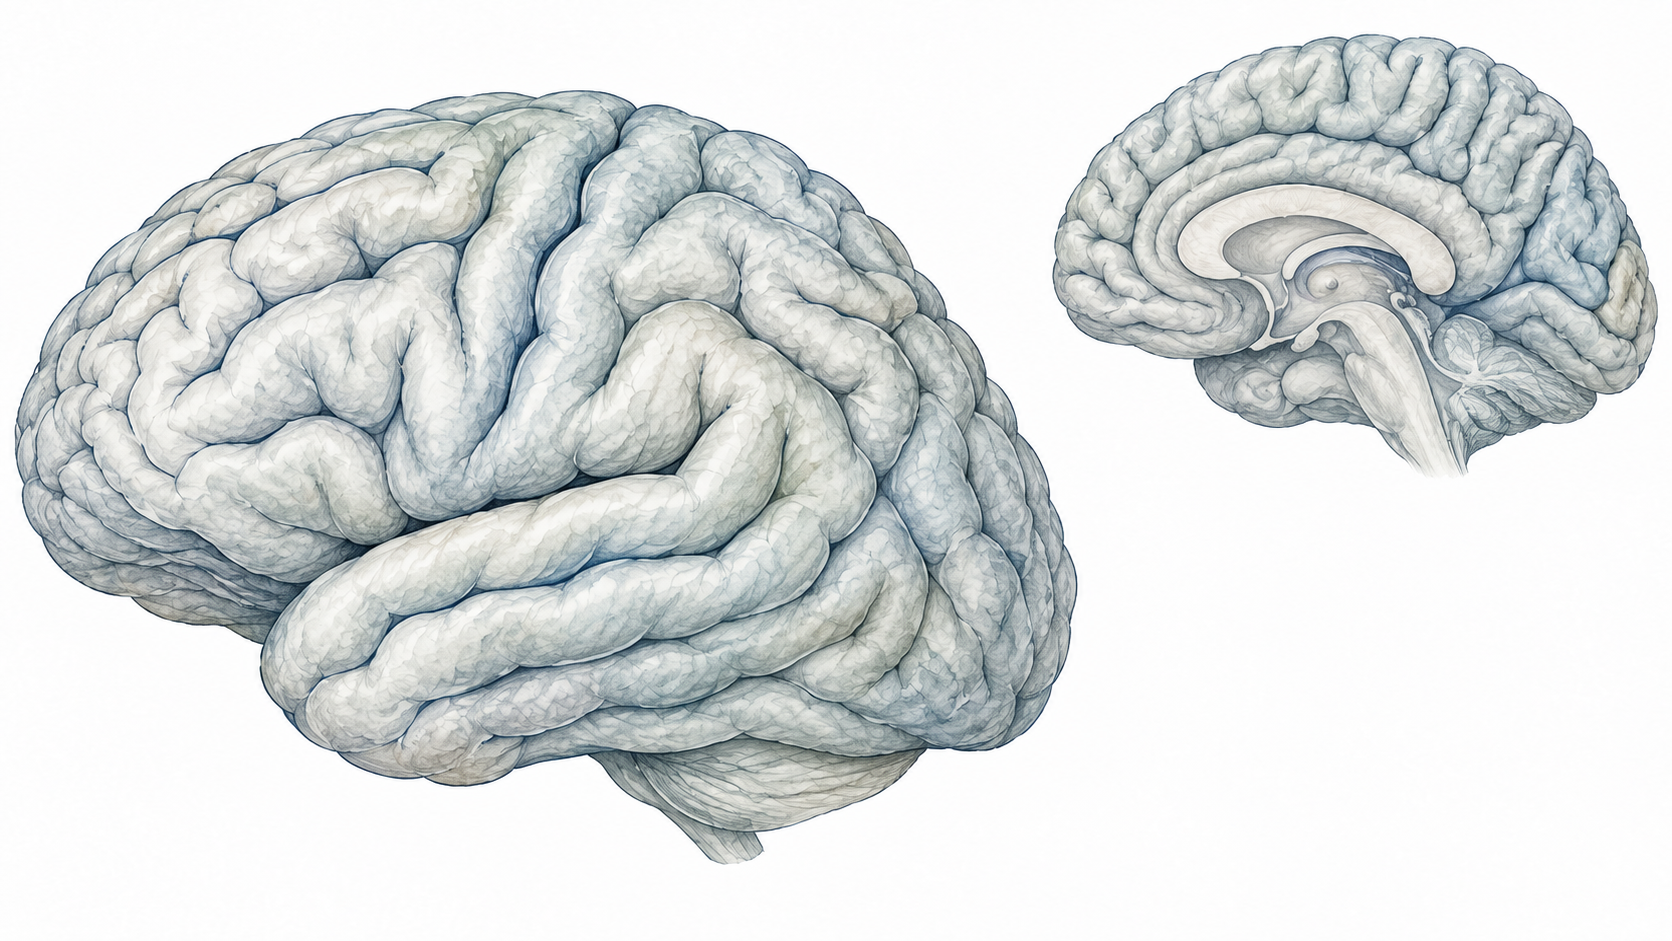
\includegraphics[width=168mm]{figures/neural-overview-brain-anatomy.png}};
  \node[anchor=west,text=BookMuted] at (1,100) {外侧视图：左为前，右为后};
  \node[text=BookMuted] at (138,100) {内侧视图};
  \node[annotation] (central) at (49,94) {中央沟};
  \draw[leader] (central.south)--(54,85)--(57,72);
  \node[annotation,text=BookMuted] at (23,66) {额叶};
  \node[annotation,text=BookMuted] at (38,34) {颞叶};
  \node[annotation,text=BookMuted] at (103,33) {枕叶};
  \node[area,draw=BookBlue] (parietal) at (74,70) {};
  \node[annotation] (parietallabel) at (81,90) {顶叶皮层};
  \draw[leader] (parietallabel.south)--(81,81)--(parietal);
  \node[area] (v1) at (103,42) {};
  \node[annotation,anchor=west] (v1label) at (111,43) {V1（内侧投影）};
  \draw[leader] (v1)--(v1label.west);
  \node[area] (v2) at (97,46) {};
  \node[annotation] (v2label) at (110,53) {V2};
  \draw[leader] (v2)--(103,49)--(v2label.west);
  \node[area] (v3) at (97,59) {};
  \node[annotation] (v3label) at (102,80) {V3（背侧）};
  \draw[leader] (v3label.south)--(99,73)--(v3);
  \node[area] (mt) at (81,42) {};
  \node[annotation] (mtlabel) at (73,32) {MT（V5）};
  \draw[leader] (mtlabel.north)--(77,38)--(mt);
  \node[area] (v4) at (90,25) {};
  \node[annotation] (v4label) at (96,7) {V4／hV4};
  \draw[leader] (v4label.north)--(94,17)--(v4);
  \node[area] (it) at (57,25) {};
  \node[annotation] (itlabel) at (47,7) {下颞皮层IT};
  \draw[leader] (itlabel.north)--(51,16)--(it);
  \draw[book arrow] (v1)--(v2);
  \draw[dorsal] (v2) to[out=105,in=-70] (v3);
  \draw[dorsal] (v3) to[out=165,in=-5] (parietal);
  \draw[dorsal] (v2) to[out=185,in=20] (mt);
  \draw[dorsal] (mt) to[out=100,in=-70] (parietal);
  \draw[ventral] (v2) to[out=-100,in=70] (v4);
  \draw[ventral] (v4) to[out=185,in=-5] (it);
  % 内侧图：距状沟的后部两岸属于 V1 的主要位置。
  \draw[BookTeal,line width=1.1pt] (151,64) to[out=-10,in=150] (163,61);
  \node[area,draw=BookTeal] (v1medial) at (159,66) {};
  \node[annotation] (v1mediallabel) at (145,76) {V1};
  \draw[leader] (v1mediallabel.south)--(150,69)--(v1medial);
  \node[annotation] (calcarine) at (145,44) {距状沟};
  \draw[leader] (calcarine.north)--(152,55)--(157,62.5);
  \draw[ventral] (119,30)--(131,30);
  \node[anchor=west,align=left,text=BookAmber] at (134,30) {内容通路what\\腹侧：物体识别};
  \draw[dorsal] (119,16)--(131,16);
  \node[anchor=west,align=left,text=BookBlue] at (134,16) {空间通路where\\背侧：空间与动作};
  \node[anchor=west,text=BookMuted] at (1,-3) {圆点表示概略位置；箭头表示主要前向联系，反馈与跨通路联系未画全。};
\end{tikzpicture}
}
  \caption{人脑视觉区域的位置与两条主要通路。自然解剖插画上的点位是教学定位，外侧图显示中央沟、顶叶皮层、MT（V5）、V3背侧部分，以及V4／hV4和下颞皮层IT的概略位置；内侧图标出距状沟附近的V1。外侧图中的V1、V2和腹侧区域采用位置投影。赭色实线表示经V4等区域向IT传递的内容通路what，蓝色虚线表示经MT、背侧视觉区向顶叶传递的空间通路where。点位与箭头依据视觉区研究和通路概括绘制，不表示精确边界、完整连接或唯一串行顺序；跨通路联系与反馈未画全。}
  \label{fig:neural-visual-pathways}
\end{figure*}

图中的区域名并非一张“每区只负责一个属性”的清单。V3是早期视觉区域之一，含有背侧与腹侧部分；V4及人脑常用的hV4名称关联于腹侧视觉区，其中的响应涉及颜色与形状等信息。MT也常称V5，运动相关响应是识别它的一项重要线索；人脑成像中的hMT+还可以包括邻近的运动相关区域，不能把这些名称当作边界完全相同的单一区域。\term{下颞皮层}（inferotemporal cortex, IT）指下部颞叶的一组视觉相关皮层，是理解物体识别通路的区域性称谓。人脑与其他灵长类的视觉区域在命名和边界上存在差别，图中保留V4、MT、IT等常见名称用于讲解，不声称它们在所有物种中逐一相同\scite{wandell2007}

区域间的联系通常概括为两条主要通路。\term{腹侧视觉通路}（ventral visual stream）从早期视觉区向V4等区域以及下颞皮层传递信息，偏重颜色、形状与物体身份，因此常称\term{内容通路}（what pathway），即帮助判断“看到的是什么”。\term{背侧视觉通路}（dorsal visual stream）联系MT、其他背侧视觉区与后部顶叶皮层，偏重运动、空间关系和视觉引导的动作，常称\term{空间通路}（where pathway）。例如，看到一个杯子时，识别它是杯子与确定伸手抓取时的位置、方向和手形，需要利用不同但相互配合的信息。where并不只表示报告静态坐标，也包含如何根据视觉控制动作；两条通路之间还会交换信息\scite{goodale1992}

\FloatBarrier
这些区域为何适合启发层次模型，还要回到单元响应。一个视觉神经元通常只对视野中某个范围内的刺激产生相应变化，这个范围称为\term{感受野}（receptive field）。感受野说明“哪些位置的输入能影响该单元”，单元的响应偏好则说明“这些位置上出现什么模式时响应更强”。Hubel和Wiesel在猫的视觉皮层中研究了对特定取向的光条或边缘敏感的细胞，并区分简单细胞与复杂细胞的感受野特征。简单细胞对亮暗位置的安排具有较明确的选择性，一些复杂细胞则能在一定位置范围内对相近取向的刺激作出响应。这些实验为局部响应及其组合提供了生物学依据；实验对象是猫，不能把全部细节直接当作人脑的逐层结构\scite{hubel1962}

局部响应经过后续回路组合，可以对更大范围、更复杂的模式产生选择性：早期视觉区中的取向信息与后续区域中的形状、物体相关响应，共同提供了理解\term{层次特征}（hierarchical feature）的生物学线索，即利用已有特征继续形成新的特征。这里的层次跨越多个回路和区域，与皮层的六个解剖层属于不同概念。视觉连接还包含反馈和并行通路，因此“局部边缘—形状—物体”适合作为理解线索，不能当作大脑必须逐步执行且只执行一次的流程\scite{purves2001}

\subsection{生物学习}
\label{sec:neural-biological-learning}

视觉回路能够组合已有响应，但经验还需要改变以后面对输入时的响应。短暂的膜电位变化描述细胞当前的状态；较持久的连接变化则能改变后续输入产生的影响。\term{突触可塑性}（synaptic plasticity）指突触传递效果能够随活动等因素改变，是研究生物学习的一类重要机制。

先看只依赖连接两端活动的简化规则。用标量$w_j$概括第$j$条连接的强度，用$u_j$和$h$分别概括输入端与输出端的活动，一个相关性更新例子是
\begin{equation}
  \Delta w_j=\eta u_j h,
  \label{eq:neural-local-correlation}
\end{equation}
其中$\Delta w_j$是连接强度的改变量，$\eta>0$控制更新幅度。这个式子展示一种\term{赫布学习}（Hebbian learning）思路：共同活动影响连接强度。它是便于比较的信息依赖示例，没有脉冲时序、权重限制和整体任务误差，不能当作完整生物学习机制；若持续出现正相关活动而没有其他约束，权重还可能不断增大。

相关活动还可以细分为发放的时间关系。\term{脉冲时序依赖可塑性}（spike-timing-dependent plasticity, STDP）描述突触变化对两端脉冲相对时刻的依赖。Bi和Poo在培养的海马神经元中观察到，特定配对条件下，突触变化与脉冲先后关系有关；该结果描述的是相应细胞和实验条件，不能直接扩成所有突触的统一规则\scite{bi1998}

局部相关性还没有解决“怎样改变连接才能改善行为”这个问题。例如，伸手抓取杯子时动作出现偏差，需要把行为结果与参与感觉和动作的多个回路联系起来。这种\term{信用分配}（credit assignment）问题关心整体结果的好坏应怎样影响内部各个环节。仅仅知道两端曾经共同活动，并不足以确定这条连接对行为偏差的贡献。生物可塑性还受到反馈和调节信号的影响，局部变化如何与整体目标联系，仍是研究的重要问题\scite{lillicrap2020}

\subsection{与人工神经网络的对比}
\label{sec:neural-biological-comparison}

生物细胞、回路和可塑性为人工模型提供了不同层次的启发。比较时需要明确当前关注的是输入与输出的函数关系、信号的时间动态，还是学习规则；同一个模型可以在某一方面相似，在另一面采用工程上的简化。

人工计算单元保留了“多个输入共同影响输出”这一抽象。若输入为$\bm{u}\in\mathbb{R}^{d}$，单元可以写为
\begin{equation}
  a=\sum_{j=1}^{d}w_j u_j+b,\qquad h=\sigma(a),
  \label{eq:neural-artificial-unit}
\end{equation}
其中$w_j$描述第$j$项输入对加权和$a$的影响，$b$调整响应的位置，$\sigma$把$a$映射为输出$h$。权重对应的是连接影响强弱的数学抽象，激活函数对应的是输入与输出之间的响应关系；二者都没有完整描述突触化学过程或细胞电生理。

图~\ref{fig:neural-unit-abstraction}把人工单元的运算展开：每项输入乘以相应权重，所有贡献与偏置相加，再经过激活函数。这种画法便于逐项核对式\eqref{eq:neural-artificial-unit}，却已经省略了图~\ref{fig:neural-biological-neuron}中的细胞形态与化学过程。该式也没有内部时间状态，因此仅凭当前$\bm{u}$就能计算$h$；一个真实细胞的响应还可能依赖此前的膜电位、近期活动和其他调节因素。这一差别决定了普通单元适合哪种抽象，也为后文保留时间动态的脉冲模型留下了空间。

\begin{figure}[htbp]
  \centering
  % 原创计算示意；权重边、偏置与正文公式逐项对应。
\begin{tikzpicture}[x=1mm,y=1mm,font=\footnotesize]
  \node[text=FigureInput] (u1) at (5,32) {$u_1$};
  \node[text=FigureInput] (u2) at (5,20) {$u_2$};
  \node[text=BookMuted] at (5,9) {$\vdots$};
  \node[text=FigureInput] (ud) at (5,-2) {$u_d$};
  \node[circle,draw=FigureModel,fill=FigureModel!12,
    minimum size=10mm,inner sep=0pt] (sum) at (45,20) {$\sum$};
  \node[book node,fill=FigureModel!12,minimum width=14mm] (activation) at (77,20) {$\sigma$};
  \node[text=FigureOutput] (output) at (105,20) {$h$};
  \node (bias) at (45,39) {$b$};
  \draw[book arrow] (u1)--node[above,sloped] {$w_1$} (sum);
  \draw[book arrow] (u2)--node[above] {$w_2$} (sum);
  \draw[book arrow] (ud)--node[below,sloped] {$w_d$} (sum);
  \draw[book arrow] (bias)--(sum);
  \draw[book arrow] (sum)--node[above] {$a$} (activation);
  \draw[book arrow] (activation)--(output);
  \node[text=BookMuted,align=center] at (45,-8) {整合输入};
  \node[text=BookMuted,align=center] at (77,-8) {产生响应};
\end{tikzpicture}

  \caption{人工神经元的计算示意。标有$w_j$的输入边表示乘以权重，求和节点再加入偏置$b$，激活函数产生输出$h$。接收输入、整合影响与产生输出，是它与生物神经元之间的功能对应；图中的数学运算不完整复现细胞机制。}
  \label{fig:neural-unit-abstraction}
\end{figure}

\Needspace{10\baselineskip}
多个单元连接起来，比较的对象便从细胞变为网络。图~\ref{fig:neural-biological-artificial-networks}左侧用局部回路与跨区域连接表示生物组织的一些特点，右侧则给出一个明确的层状前馈计算。右图的中间输出按约定次序计算，左图所示回路则可以让此前活动再次影响后续响应。人工网络也可以加入反馈、状态和不同单元类型；二者的区别需要落实到具体结构与动态，而不能只看图上都有节点和连线。一个生物神经元可以具有复杂的树突计算，一个人工单元也可以被设计成复杂函数，因此神经元数、人工单元数与参数量不能直接互换。

\begin{figure}[htbp]
  \centering
  % 原创教学拓扑；左图不是实测脑连接，右图是有限前馈计算依赖。
\begin{tikzpicture}[x=1mm,y=1mm,font=\footnotesize,
  cell/.style={circle,draw=FigureModel,fill=FigureModel!12,minimum size=4mm,inner sep=0pt},
  othercell/.style={rectangle,rounded corners=0.5mm,draw=FigureModel,fill=BookPaper,minimum size=4mm,inner sep=0pt},
  link/.style={book arrow,line width=0.5pt}]
  \node[font=\heiti\small] at (23,52) {生物神经网络的局部示意};
  \node[font=\heiti\small] at (86,52) {前馈人工神经网络};
  \path[fill=BookBlue!7,rounded corners=3mm] (1,26) rectangle (23,45);
  \path[fill=BookTeal!7,rounded corners=3mm] (27,15) rectangle (48,38);
  \path[fill=BookAmber!7,rounded corners=3mm] (3,1) rectangle (25,20);
  \foreach \i/\x/\y in {1/6/38,2/18/39,3/12/30,4/31/29,5/42/32,6/39/20,7/8/10,8/19/13}{
    \node[cell] (b\i) at (\x,\y) {};
  }
  \node[othercell] (b9) at (13,4) {};
  \foreach \i/\j in {1/2,2/3,3/1,4/5,5/6,6/4,7/8,8/9,9/7,3/4,6/8,7/3}{
    \draw[link] (b\i)--(b\j);
  }
  \draw[link] (b5) to[bend right=38] (b2);
  \node[text=BookMuted,align=center] at (23,-9) {局部回路与跨区域联系\\细胞保留内部动态};
  \foreach \i/\y in {1/8,2/23,3/38}{
    \node[cell,draw=FigureInput,fill=FigureInput!12] (x\i) at (65,\y) {};
  }
  \foreach \i/\y in {1/8,2/23,3/38}{\node[cell] (h\i) at (85,\y) {};}
  \foreach \i/\y in {1/15,2/31}{
    \node[cell,draw=FigureOutput,fill=FigureOutput!12] (o\i) at (105,\y) {};
  }
  \foreach \i in {1,2,3}{\foreach \j in {1,2,3}{\draw[link] (x\i)--(h\j);}}
  \foreach \i in {1,2,3}{\foreach \j in {1,2}{\draw[link] (h\i)--(o\j);}}
  \node[text=BookMuted] at (65,0) {输入};
  \node[text=BookMuted] at (85,0) {表示};
  \node[text=BookMuted] at (105,0) {输出};
  \node[text=BookMuted,align=center] at (86,-9) {按层传递数值\\依计算次序求值};
\end{tikzpicture}

  \caption{从单元到网络的两种组织示意。左侧用轮廓不同的节点表示细胞类型差异，淡色区域表示局部群体，箭头同时包含局部回路与跨群体联系；它是教学构造，并非测得的人脑连接图。右侧是一个前馈人工网络，箭头表示输入、中间表示与输出之间的计算依赖。图中的节点数量不表示真实规模，右图也不涵盖人工网络的所有结构。}
  \label{fig:neural-biological-artificial-networks}
\end{figure}
\FloatBarrier

前面介绍的视觉感受野与层次响应，带来了一个人工视觉模型的设计问题：能否在不同位置检测局部模式，再把这些检测结果组合成更大范围的表示？Fukushima在1980年提出的\term{新认知机}（neocognitron）受这种层次思路启发，交替组织检测局部模式的S单元与汇集响应的C单元，以获得对位置变化具有一定容忍度的识别表示。这是从视觉机制走向人工层次结构的一项早期工作，其自组织学习方法也与后来的监督梯度训练不同\scite{fukushima1980}

卷积神经网络沿用的核心设计包括局部感受野、重复使用局部检测方式，以及逐层扩大信息组合范围。局部连接限制一个单元读取的输入区域；参数共享则把同一个检测函数用于不同位置。后者是明确的工程约束，不能从“许多生物细胞具有相似响应偏好”推出它们精确共享同一组突触参数。网络还可以采用\term{池化}（pooling），即汇总邻域内的若干响应，以降低表示的空间分辨率或减小对局部位移的敏感性。卷积、非线性响应与邻域汇总组合后，后层能够读取较大范围内的局部特征组合。

这些联系说明了卷积网络为什么适合从局部结构构造视觉表示，并不要求某个卷积层恰好对应V1、下一个层对应V2。what与where也区分了表示服务的目标：物体识别希望在位置变化后仍保留身份判断，定位和动作控制却需要保留空间关系，不能一概消除位置信息。后面的卷积神经网络章将把感受野、参数共享、池化以及平移等变与不变的条件写成明确运算；这里的生物学关联为这些设计提供动机，其性质仍需由具体计算和证据来判断。

\term{脉冲神经网络}（spiking neural network, SNN）把单元之间传递的信号表示为离散脉冲事件，并通常保留随时间演化的内部状态。它既可用于研究神经系统，也可用于任务预测和事件驱动计算；连接结构、单元动态和参数学习规则还需要分别设计。

脉冲模型可以用输入改变膜电位、达到阈值时发放并重置状态等规则，保留“积累—发放”的时间过程；普通连续值单元则常直接计算当前输入对应的数值。这样的差别使SNN更适合表达某些脉冲时刻相关的问题，但脉冲编码不自动补齐树突形态、递质作用、胶质支持或生物可塑性。卷积与脉冲也不是互斥的网络类别：前者规定局部连接和参数共享，后者规定信号形式与时间动态，因而可以构造采用脉冲单元的卷积网络\scite{gerstner2014}

\paragraph{学习机制与信用分配}
在单元形式之外，更深的差别是怎样从经验中改变连接。常见的人工网络训练直接规定一个整体损失，并利用该损失对各参数的导数更新参数。对于式\eqref{eq:neural-artificial-unit}，设当前可微损失$\mathcal{L}$通过输出$h$依赖权重$w_j$，则
\begin{equation}
  \frac{\partial\mathcal{L}}{\partial w_j}
  =\frac{\partial\mathcal{L}}{\partial h}\,\sigma'(a)\,u_j\text{。}
  \label{eq:neural-unit-credit}
\end{equation}
输入$u_j$和局部导数$\sigma'(a)$只描述这个单元附近的计算；$\partial\mathcal{L}/\partial h$还包含$h$通过后续网络影响损失的信息。\term{误差反向传播}（error backpropagation）从输出端出发，沿计算依赖反向应用链式法则，组织这些导数的计算。它提供梯度；用梯度怎样修改参数，是优化算法的工作。若激活函数在某点不可微，则需另行约定该点的处理方式。

\Needspace{7\baselineskip}
两类学习的共同点，是经验能够改变连接的影响，进而改变下一次输入引起的响应。生物突触的传递效果与人工权重都承担了这种作用，许多连接的变化共同影响网络的行为。这里还需要区分当前活动与连接学习：一次脉冲或一次前向计算改变当前活动，连接学习则改变突触传递效果或模型参数。内部状态也可以保存信息，但状态变化与连接更新是不同的对象。这个对应解释了为什么人工网络可以借鉴可塑性，却没有规定两者必须使用同一种更新规则。

生物学习的重要基础是局部突触可塑性。通常所说的\term{赫布定律}（Hebb's rule）强调：一个神经元的活动反复参与另一个神经元的发放，两者之间的连接可能增强。式\eqref{eq:neural-local-correlation}展示的是这种思想的简化形式。不过，大脑的学习不能只写成“两端同时活动就增强连接”。脉冲时序、细胞状态与调节信号都会影响变化；一些研究还考察局部活动能否先留下短暂的突触痕迹，待奖励等信号到来时再改变连接。这使局部活动能够与稍后出现的行为结果联系起来，仍不等于逐条计算整体损失的精确梯度\scite{gerstner2018plasticity}

最关键的不同点，是更新依据什么信号，以及这个信号怎样到达内部连接。标准反向传播把一个明确的任务损失作为共同依据：式\eqref{eq:neural-unit-credit}中的$\partial\mathcal{L}/\partial h$衡量隐藏输出如何影响最终损失，后续计算的导数又把这一影响传回当前单元。因此，即使两条连接附近的活动相似，只要它们对任务误差的贡献不同，得到的梯度也可以不同。式\eqref{eq:neural-local-correlation}仅使用两端活动，STDP则进一步利用脉冲的相对时刻；这些局部量本身没有给出最终任务损失的精确导数。用“活动相关”决定变化，与用“对任务误差的影响”决定变化，是本节两种更新示例最需要区分的地方。

学习信号的实现方式也不同。在常见的软件实现中，人工网络沿已知计算图反向求导，并在数值存储中更新参数；生物突触的变化由细胞内过程实现，能够使用的活动、时序及反馈信号受实际连接和动态限制。\textbf{目前不能把大脑的学习机制等同于标准反向传播，也不能用单一赫布规则概括全部生物学习。}大脑存在广泛反馈，研究仍需解释这些反馈怎样帮助信用分配。Lillicrap等讨论了利用反馈引起的活动变化近似误差信号的可能机制；这是关于可能实现方式的探索，尚不构成大脑执行标准反向传播的证据\scite{lillicrap2020}

上述差异针对本节比较的局部可塑性与标准反向传播，不是生物和人工系统的绝对分界。人工网络也可以采用局部相关性更新，脉冲网络也可以按任务损失训练。采用哪种编码、怎样连接单元、怎样学习参数，是需要分别说明的设计选择。

\paragraph{信息流动与自上而下的预测}
学习规则不同，还要与感知时的信息流区分开。在一个普通前馈分类器中，输入经过各层产生输出，一次预测不需要把高层结果再送回低层。人脑的视觉系统则同时存在自下而上的感觉输入和自上而下的反馈，当前理解会反过来影响对输入的处理。Bar等的研究支持一种具体假说：图像的粗略信息较快到达额叶中的眶额皮层，由这里形成可能的物体解释，再帮助颞叶视觉区域识别输入。研究观察到识别相关的眶额活动早于相应颞叶活动，这为预测参与视觉识别提供了依据；不能据此把所有预测都归结为额叶一个区域\scite{bar2006}

面对模糊物体时，已有经验可以帮助形成候选解释，再与当前感觉证据相互校正。日常所说的“脑补”可以从这种补全缺失信息的过程理解；预测可能帮助识别，也可能使错误预期干扰判断。\textbf{感知中的反馈传递神经活动，反向传播计算训练所需的导数，两者是不同过程。}人工网络也能加入循环、反馈或反复推断，因此“人工信息流只有前向”只适用于这里比较的前馈结构，不能概括全部人工架构。

\paragraph{少样本学习与知识迁移}
人往往能利用少量新例子理解与已有经验相关的概念。例如，已经熟悉书写的人看到一个陌生字符，可以利用笔画、连接和书写方式来判断它的其他写法。Lake等以手写字符为对象研究单样本概念学习，并构造了能够组合和复用笔画等知识的程序模型；模型在相应任务上达到与人类相近的表现。这项结果说明，少量新样本可以与丰富的已有知识共同支持泛化，而不是证明人脑在毫无先前经验时也能学会任意任务\scite{lake2015}

相比之下，从随机参数开始、针对固定类别训练的监督网络，常需要较多带标签样本才能形成相应表示；它不能自动获得人已积累的概念与经验。人工网络也可以通过迁移学习复用表示，或通过元学习练习如何用少量数据适应新任务，前文的字符学习例子已说明这种组织方式\scite{finn2017}比较样本效率时，需要同时记录新任务用了多少样本，以及此前用了多少数据、任务和其他知识。人类的快速迁移是人工学习的重要参照，但新知识与旧知识的联系越弱，就越不能假定只需少量练习。

\paragraph{鲁棒性与对抗扰动}
在熟悉对象的识别中，人可以容忍一定程度的模糊、遮挡和背景变化。不过，普通图像上的高准确率并不保证人工网络也具有同样的感知稳定性。Szegedy等发现，针对网络寻找的细小图像扰动，可以在视觉上几乎不改变图像时使模型误分类\scite{szegedy2014intriguing}例如，可以出现人仍把图像看作一个杯子，分类器却输出另一类别的情形。这里的扰动经过有意搜索，与随意加入一点随机噪声不同；它暴露了模型的分类依据与人的判断之间的差距。

\Needspace{7\baselineskip}
\textbf{人眼不易察觉的扰动能使某些模型出错，不等于人脑对所有对抗攻击都免疫。}Elsayed等发现，在限制观察时间的实验条件下，一些针对计算机视觉系统构造的扰动也会影响人的分类\scite{elsayed2018humans}人类还会受到错误预期和跨感官冲突的影响。因此，比较鲁棒性应固定任务、扰动范围、观察时间和评价指标；人工网络的稳健训练也会改变结果。
\BookChapterRef{chap:trust-robustness}{第二卷“基础、理论和可信性”的“鲁棒性”章}
已经说明，普通噪声、自然分布变化与主动寻找的最不利扰动需要分别评价。

\paragraph{计算活动的能量成本}
人脑在约$20\,\mathrm{W}$量级的代谢功率下，持续维持感觉、行动和内部活动，这种丰富功能与较低功率并存的现象构成了人工计算的重要参照。这个数字包含通信和维持细胞功能等成本，不能只算作“有用运算”的功率；脑内的信息传递本身也需要能量\scite{levy2021}典型数字实现中的人工网络则要执行数值运算，并在存储与计算部件之间读取权重和中间结果。模型大小、计算精度、活动是否稀疏以及数据搬运方式，都会影响实际能耗。

生物回路中的稀疏脉冲活动和局部连接为减少不必要的计算和通信提供了设计线索，但采用脉冲模型并不自动保证节能。比较时还要区分功率与能量：同样的功率，运行时间越长，总能量越多。因而，不能用整个人脑的代谢功率直接对比某块设备的额定功率，就得到每次判断的能效倍数；应固定任务与准确率，并计入响应时间、学习成本以及所测系统的范围。

\paragraph{多感官输入与联合处理}
听别人说话时，声波和说话者的口形同时提供线索。人脑可以联合处理这些输入，而不是等视觉和听觉各自给出最终答案后才简单拼接。这种\term{多模态处理}（multimodal processing）利用不同类型的信息通道共同理解同一事件。McGurk和MacDonald的经典实验表明，把一种音节的声音与另一种音节的口形配在一起，会使一些人报告听到第三种音节，说明视觉信息能够改变语音感知，而不只是给听觉附加一条独立说明\scite{mcgurk1976}

神经系统本身具有多种感觉通道及跨通道联系，具体整合能力仍会随发育和经验形成，不能把所有跨感官关联都理解为出生时已经成熟\scite{stein2014multisensory}许多人工模型只为一种输入类型设计，需要另外建立不同输入之间的联系；人工网络也能学习多模态表示。例如，图像与文本的联合训练可以把描述和图像关联起来\scite{radford2021}这里的差别在于系统能够利用哪些输入、哪些关联来自结构或经验，以及训练是否建立了这些关联，并非人工网络原则上只能处理单一模态。

应当保留多少生物细节，取决于模型要回答什么问题。面向预测的人工网络主要用任务表现评价，不必让每个模块对应真实脑区。解释神经系统的模型则要对应特定观察：研究脉冲时间，需要保留影响发放的动态；解释突触变化，需要说明更新规则与实验条件的关系。简化后的结论只能覆盖保留下来的机制，复现某组神经响应也不能单凭这一点确定学习过程相同。

这些方向可以相互借鉴，但预测准确率、生物解释与运行代价是不同的评价标准。在其中一项上有效，不等于另外两项也有证据支持。后续介绍人工架构时，我们将明确其计算假设；涉及生物机制时，再检查所保留的细节与结论范围。

\section{神经网络的历史}
\label{sec:neural-history}

表示、参数学习和计算资源是相互配合的：能够写出一个复杂网络，并不等于知道怎样训练它；有了梯度，也不等于能够在有限资源下处理所需数据。沿着这三个问题考察历史，比只记模型名称和年份更能说明技术变化带来了什么。本节选取与后续架构直接有关的工作，年份指所述论文的发表或首次公开时间。

\subsection{从阈值单元到可学习网络}
\label{sec:neural-history-threshold}

1943年，McCulloch和Pitts用理想化的二值神经元研究神经活动与逻辑计算的关系。单元根据输入和阈值决定是否活动，多个单元连接后可以表达逻辑关系。这项工作建立了用简单单元及其连接描述计算的早期形式化框架，其中心问题是计算如何由网络实现，而不是用现代的训练目标从数据中优化全部参数\scite{mcculloch1943}

当连接权重也允许根据样本改变，研究问题就从“怎样构造计算”延伸到“怎样获得所需计算”。Rosenblatt在1958年的感知机研究中讨论了从经验形成识别行为的网络。前文介绍的基础感知机是这一思路的简化形式：对输入加权求和，按阈值分类，再根据分类错误调整权重。历史上的感知机系统还包含输入与中间组织，不能把原始工作中的所有网络形式都归为今天常用的单层线性分类器\scite{rosenblatt1958}

基础感知机的限制可以由示例~\ref{ex:neural-xor-representation}直接看出：若输入只有$x_1,x_2$，调整线性得分的参数无法表示异或。改变输入特征或加入非线性隐藏层，则改变了允许表达的函数。因此，“单层线性分类器不能表示异或”与“神经网络不能表示异或”是不同命题。隐藏层补上了表示能力，接下来还需解决如何根据最终输出学习隐藏层参数的问题。

\subsection{从浅层学习到深层训练}
\label{sec:neural-history-deep-training}

隐藏层没有直接给定的目标值，难以像输出层那样根据标签判断每个单元应该输出什么。1986年，Rumelhart、Hinton和Williams展示了通过反向传播误差训练多层网络、形成内部表示的方法。最终目标对隐藏活动的影响可以通过链式法则计算，因而不必为每个隐藏单元人工指定答案。这项工作说明了多层表示怎样参与学习；这里并不把1986年说成链式求导或所有相关算法的首次出现\scite{rumelhart1986}

有了参数学习方法，连接结构仍然影响模型怎样利用数据。卷积网络在规则网格上组合局部信息，并在不同位置共享参数；LeCun等1998年的文档识别研究展示了这种结构与基于梯度的整体学习如何结合。手写字符在不同位置出现时，网络可以重复使用已经学习到的局部检测方式，无需为每个位置重新估计一套完全独立的参数\scite{lecun1998}

对序列，关键问题是怎样利用此前输入。循环结构把历史信息写入状态，再将状态用于下一步计算。但信息与梯度经过许多更新后可能衰减。Hochreiter和Schmidhuber在1997年提出\term{长短期记忆}（long short-term memory, LSTM），通过记忆路径和可学习的门控制信息的写入与读取。这个名称指一种具体循环网络结构，其目的与机制都涉及跨时间的信息保留，不表示所有长期依赖都会自动被学会\scite{hochreiter1997}

深层模型能否发挥作用，还取决于数据规模和计算实现。Krizhevsky、Sutskever和Hinton在2012年的ImageNet分类研究中，结合大规模标注图像、图形处理器上的训练、非线性单元和防止过拟合的训练设计，展示了深层卷积网络的任务表现。这一例子说明，结构、学习方法、数据与计算条件能够共同改变可实现的模型规模；它不能归结为“增加层数就一定提高准确率”\scite{krizhevsky2012}

这些工作没有形成一条“旧模型被新模型完全取代”的路线。卷积利用空间结构，循环保留序列状态，层次变换构造表示，梯度计算支持参数学习，它们解决的是不同问题，也可以组合使用。后续章节将分别检验各项假设、机制和适用条件。

\subsection{从固定连接到内容相关计算}
\label{sec:neural-history-content-dependent}

局部连接预先规定单元读取哪些位置，固定长度的序列状态则把历史压缩进同一组数值。当当前预测只需要历史中的某一部分时，模型还可以根据当前内容决定读取什么。\term{注意力机制}（attention mechanism）为候选信息计算相关性权重，再用这些权重组合信息。它改变的是本次计算中各信息来源的影响，而不要求把全局模型参数临时重新训练。

Bahdanau、Cho和Bengio在2014年公开、2015年发表于ICLR的机器翻译研究中，让解码过程按当前需要读取输入序列不同位置的表示。编码器不再只提供一个固定长度的整体概括，而是保留各位置的表示供解码器动态聚合。注意力由此可以与循环网络配合，缓解单一整体表示带来的信息读取限制\scite{bahdanau2015}

2017年的\term{Transformer}架构以注意力为主要信息交互机制，并组合逐位置变换等模块。在\term{自注意力}（self-attention）中，同一组输入中的各位置根据彼此内容交换信息；给定一整段已知输入，许多位置的计算可以并行组织，不需要像普通循环编码器那样先逐步构造全部状态。生成序列时，尚未产生的内容仍然不可用，因此并行训练的计算形式不能直接推出整个生成过程同时完成\scite{vaswani2017}

内容相关计算还可以决定使用哪些计算模块。\term{条件计算}（conditional computation）根据输入选择本次启用的部分路径；\term{混合专家}（mixture of experts, MoE）则用多个子网络共同提供候选变换，并由路由机制选择或加权组合它们。Shazeer等2017年的稀疏门控工作让每个输入只使用部分专家，区分了网络存储的总参数与一次输入实际参与计算的参数。路由、负载分配和数据传递也有代价，不能仅由激活专家少就断定总体运行成本低\scite{shazeer2017}

另一条路线继续保留状态递推，同时改进状态的组织与计算。\term{状态空间模型}（state space model, SSM）用状态描述此前输入对后续输出的影响。用于序列的神经网络可以把这种更新嵌入可学习模块；2021年公开、2022年发表于ICLR的\term{结构化状态空间序列模型}（structured state space sequence model, S4）通过特定的状态矩阵组织计算，在线性、时不变等条件下联系递归更新与卷积计算\scite{gu2022s4}2023年公开的Mamba进一步让部分更新量依赖当前输入，使状态保留和遗忘具有内容选择性\scite{gu2023mamba}

这段发展改变了理解网络时需要观察的对象。除了参数和固定拓扑，还应考察本次输入决定的注意力权重、所选择的模块，以及随输入演化的状态。它们都是运行中的计算量或活动，不必等同于训练后保存的全局参数。状态空间网络与循环网络的联系、自注意力与消息传递的联系，也说明现代架构的差别需要按具体机制判断。

\section{神经网络的类型}
\label{sec:neural-network-types}

“卷积”“循环”“图”“注意力”“脉冲”分别强调不同性质。将这些名称并排列出，容易误以为一个网络只能属于其中一类。本节按连接结构、信息交互方式和信息编码方式分别观察同一个计算对象；这些分类可以交叉，也不要求每个完整架构只使用一种机制。

\subsection{按连接结构划分}
\label{sec:neural-types-connectivity}

连接结构关心计算单元之间的依赖方向与组织方式。\term{前馈神经网络}（feedforward neural network）沿没有有向环的计算依赖，把输入逐步送到输出；同一次计算中的中间结果不再返回去修改自己的上游输入。式\eqref{eq:neural-layer-composition}是层状前馈网络，跨层连接也可以保持前馈性质，只要计算依赖仍然没有有向环。

\term{循环神经网络}（recurrent neural network, RNN）把此前状态用于下一次更新。同一组更新参数在多个时间步重复使用，因而既处理当前输入，也传递历史影响。固定输入序列并按时间展开后，每一步读取已计算出的前一步状态，得到的展开计算可以没有有向环；名称中的“循环”描述的是状态反馈与参数复用，不是要求在一个时间步中无限反复求值。

例如，判断一句评论是肯定还是否定，可以先把整句转为定长向量，再让前馈网络逐层得到分类得分；也可以让循环网络逐词读取评论。后一种结构在读到“不”后更新状态，读到“好”时同时使用当前词和此前状态，因而提供了保留否定关系的途径。前馈结构传递的是本次计算中已经得到的中间值，循环结构还显式传递跨时间步的状态；存在这条状态通道，并不保证训练后就一定记住了“不”。

依赖也可以沿树组织。\term{树递归网络}（recursive neural network）按照树中的父子关系递归地组合表示，例如用两个子树的表示形成父节点表示。链式状态更新每次通常接收一个前序状态，树递归则可能组合多个子节点状态，计算顺序和共享方式因此不同。本书采用广义的循环网络口径，把链式循环、树递归及基于隐状态递推的状态空间网络放在循环网络章讨论；它们的具体拓扑仍分别说明。

\term{图神经网络}（graph neural network, GNN）根据输入图中的实体和关系组织表示计算，例如让一个节点读取相邻节点的信息。这里必须区分输入图与网络的计算依赖：输入图可以有环，模型却可以只执行固定轮数的同步更新，时间或轮次展开后仍得到有限的计算过程。另一类图网络通过反复状态更新求取某种稳定状态，两者的学习和计算条件不同。

以预测路口拥堵为例，输入节点可以是路口，边表示道路连接。一次同步更新让每个路口读取上一轮的邻居车流表示，再生成自己的新表示。即使道路形成环路，这一轮也不用等待邻居先算出同一轮的新值；按轮次保存旧值与新值，就能执行有限次更新。

图~\ref{fig:neural-topologies}将三个常见依赖模式放在一起。前馈图说明层间先后，链式展开说明状态的跨时间依赖，输入图则说明哪些实体有关联。每个神经网络都能用计算图描述，不意味着每个网络都是图神经网络；后者的“图”特指模型利用输入的关系结构来组织计算。

\begin{figure}[htbp]
  \centering
  % 原创示意。左：计算依赖；中：时间展开；右：数据关系图。
\begin{tikzpicture}[x=1mm,y=1mm,font=\figurefont\footnotesize,
  unit/.style={circle,line width=1.1pt,minimum size=3.5mm,inner sep=0pt,draw=NNHidden,fill=NNHidden!18}]
  \node[font=\figurefont\bfseries\small] at (15,34) {前馈计算};
  \node[font=\figurefont\bfseries\small] at (60,34) {循环的时间展开};
  \node[font=\figurefont\bfseries\small] at (99,34) {输入关系图};
  \foreach \i/\y in {1/5,2/17,3/29}{
    \node[unit,draw=NNInput,fill=NNInput!18] (x\i) at (2,\y) {};
  }
  \foreach \i/\y in {1/9,2/25}{\node[unit] (h\i) at (15,\y) {};}
  \node[unit,draw=NNOutput,fill=NNOutput!18] (o) at (28,17) {};
  \foreach \i in {1,2,3}{\foreach \j in {1,2}{\draw[nn legacy arrow] (x\i)--(h\j);}}
  \foreach \j in {1,2}{\draw[nn legacy arrow] (h\j)--(o);}
  \foreach \i/\x/\state/\input in {
    1/42/{\bm{s}^{(t-1)}}/{\bm{x}_{t-1}},
    2/60/{\bm{s}^{(t)}}/{\bm{x}_{t}},
    3/78/{\bm{s}^{(t+1)}}/{\bm{x}_{t+1}}}{
    \node[unit,minimum size=5mm] (s\i) at (\x,18) {};
    \node[above=2mm of s\i] {$\state$};
    \node (u\i) at (\x,2) {$\input$};
    \draw[nn legacy arrow] (u\i)--(s\i);
  }
  \draw[nn legacy arrow] (s1)--(s2);
  \draw[nn legacy arrow] (s2)--(s3);
  \foreach \i/\x/\y in {1/94/8,2/104/8,3/99/24,4/110/26}{
    \node[unit,draw=NNInput,fill=NNInput!18] (v\i) at (\x,\y) {};
  }
  \draw[nn link] (v1)--(v2)--(v3)--(v1);
  \draw[nn link] (v3)--(v4);
\end{tikzpicture}

  \caption{三种不同对象的结构示意。左侧是前馈计算中的单元依赖；中间是循环更新的时间展开，三个更新位置共享同一组状态更新参数；右侧是供图神经网络使用的输入关系图，节点表示数据中的实体，边表示输入中的关系。右图的无向环不等于一次计算中的循环依赖。}
  \label{fig:neural-topologies}
\end{figure}
\FloatBarrier

\subsection{按信息交互方式划分}
\label{sec:neural-types-interaction}

确定了大体依赖后，还需说明一次更新怎样组合信息。\term{全连接}（fully connected）让一组输出中的每个单元读取上一组的全部坐标，常用一个稠密矩阵完成加权组合。\term{卷积}（convolution）则按规则网格读取局部邻域，并在不同位置重复使用同一组参数。全连接提供广泛的坐标组合，卷积把局部性与位置间复用直接写进运算；它们既可以构成完整网络，也可以成为同一个网络中的不同模块。

例如，要检测图像一行中相邻像素的亮度变化，可以对数值$(1,2,4,3)$依次计算相邻两项之差，得到$(-1,-2,1)$。三个位置都使用“左值减右值”这一组局部权重，而不是各学一套权重，这展示了卷积的局部共享方式。全连接层则可以让每个输出同时读取四项亮度，并各自学习四个输入权重。两种计算都能从输入向输出执行，因而“前馈”并不能决定采用哪一种交互。

在不规则关系图上，\term{消息传递}（message passing）让节点接收并聚合相邻节点的信息，再更新自己的表示。沿用路口例子，可以先对相邻路口的车流表示取平均，再与本路口的表示共同计算新值。与规则网格上的卷积相比，它由输入图决定邻域，节点的邻居数量可以不同。若用注意力根据当前车流表示计算不同邻居的贡献，就把固定的等权平均改为内容相关的加权组合。此时消息传递与注意力同时出现：前者规定参与交互的关系范围，后者规定当前输入下各关系的相对影响。

注意力还可以让一组位置在指定的可见范围内直接相互读取。卷积核的共享参数在推理时通常保持固定，注意力的聚合权重则根据当前表示计算。这里比较的是聚合方式；一个卷积网络也可以加入注意力模块，一个Transformer也包含注意力之外的前馈变换。因此，“以注意力为主”不表示全部计算都是注意力。

状态空间更新通过内部状态累积历史影响。一个离散、线性、时不变的基础形式是
\begin{equation}
  \begin{aligned}
    \bm{s}^{(t)}&=\bm{A}\bm{s}^{(t-1)}+\bm{B}\bm{x}_t,\\
    \bm{o}_t&=\bm{C}\bm{s}^{(t)}+\bm{D}\bm{x}_t,
  \end{aligned}
  \label{eq:neural-basic-state-space}
\end{equation}
其中$\bm{x}_t\in\mathbb{R}^{d}$是第$t$步输入，$\bm{s}^{(t)}\in\mathbb{R}^{m}$是状态，$\bm{o}_t\in\mathbb{R}^{r}$是输出，递推从给定的$\bm{s}^{(0)}$开始。矩阵$\bm{A}\in\mathbb{R}^{m\times m}$、$\bm{B}\in\mathbb{R}^{m\times d}$、$\bm{C}\in\mathbb{R}^{r\times m}$和$\bm{D}\in\mathbb{R}^{r\times d}$在这组公式中不随$t$改变。该线性模块可以与非线性变换组合成神经网络，输入相关更新则改变了这里的时不变假设。并行计算与递归计算能否互换，需要检查具体更新形式，不能从“状态空间”这一名称直接推出。

这些交互方式分别决定读取范围、参数如何复用、权重是否由当前内容产生，以及历史如何保留。它们与上一小节的连接分类并不是同一维度：卷积常用于前馈结构，消息传递可以按固定轮数前馈，也可以反复更新状态；状态空间模块则可以在多个层之间堆叠。判断计算代价和表达限制时，需要同时说明具体机制与组织方式。

\subsection{按信息编码方式划分}
\label{sec:neural-types-encoding}

前面的式子大多用实数向量记录单元活动。\term{连续值激活}（continuous-valued activation）用数值的大小表达当前响应，信息通过这些数值之间的运算传递。这里的“连续值”描述数学表示；计算机中的浮点数和量化数仍是有限精度编码，不能把数学上的实数模型与实际数值存储混为一谈。

脉冲编码则用离散事件及其发生时刻表达信息。例如，在固定观察窗口内，脉冲数量可以反映响应强弱；也可以用首次发放时间或多个脉冲的相对时刻表达差异。后一种读法把时间本身纳入表示，不能只用窗口内的计数代替。具体如何编码输入、维护内部状态与读取输出，需要同神经元动态一起设计。

同一个图像分类任务可以采用不同编码。假设某像素的归一化强度为$0.6$，连续值输入直接传递这个数；一种教学用计数编码把观察窗口分成$10$个时隙，其中$6$个时隙各发放一次脉冲，读取端再用计数除以$10$还原$0.6$。这个例子只约定数量，不约定哪六个时隙发放；若模型还利用事件时刻，就必须进一步指定时间安排。无论采用哪种编码，都仍可以让单元读取局部像素并共享参数，所以编码方式与卷积交互不是二选一。

两种编码可以对应相近的任务，却改变了计算和学习所需处理的对象。连续值网络可以直接对整组数值做矩阵运算；事件驱动实现可以在事件到来时处理相应更新，但也可能需要维护没有发放脉冲的单元状态。发放事件的离散性还使普通导数的使用遇到困难，需要专门的学习方法。是否节省运行代价，取决于事件密度、实现方式和硬件，不能仅由编码名称判断。

表~\ref{tab:neural-cross-classification}用三个已经解释的维度比较代表形式。表中的描述限定了相应结构，而不是给所有同名变体统一贴标签。一个采用脉冲编码的卷积网络同时具有局部共享运算和事件信号；一个带注意力的循环网络则同时具有状态递推和内容相关聚合。这些组合保留了各维度的意义。

\begin{table*}[htbp]
  \centering
  \small
  \begin{tabularx}{\linewidth}{@{}>{\RaggedRight\arraybackslash}p{45mm}>{\RaggedRight\arraybackslash}p{42mm}>{\RaggedRight\arraybackslash}X>{\RaggedRight\arraybackslash}p{26mm}@{}}
    \toprule
    \textbf{代表形式} & \textbf{连接组织} & \textbf{主要交互} & \textbf{信号编码} \\
    \midrule
    层状全连接网络 & 层间前馈 & 稠密加权组合 & 连续值激活 \\
    前馈卷积网络 & 层间前馈 & 局部连接与参数共享 & 连续值激活 \\
    带注意力的循环网络 & 状态递推 & 状态更新与动态聚合 & 连续值激活 \\
    固定轮数的图消息传递网络 & 按轮次展开 & 按输入图聚合邻居 & 连续值激活 \\
    前馈脉冲卷积网络 & 层间前馈，单元保留状态 & 局部连接与参数共享 & 脉冲事件 \\
    \bottomrule
  \end{tabularx}
  \caption{同一个网络可以同时按三个维度描述。连接组织回答计算怎样依赖，交互方式回答信息怎样组合，编码方式回答单元传递什么信号。列出的形式用于展示分类交叉，不穷尽各类网络的变体。}
  \label{tab:neural-cross-classification}
\end{table*}

\FloatBarrier
\section{本章小结}
\label{sec:neural-overview-summary}

神经网络把特征构造纳入可学习的计算路径。异或例子说明，原始坐标中的线性限制可以通过非线性中间表示改变，输出端仍可使用简单规则。多个单元共同编码信息、多个层继续组合表示，为这种变换提供了两种互补的组织方式。表示是否适合任务，则由输入信息、结构假设、学习目标与算法共同决定。

生物启发提供了单元、连接和可塑性的出发点；视觉感受野与层次组合进一步解释了局部连接的设计动机。腹侧与背侧通路还提示，物体身份与空间动作需要的表示并不相同。生物比较还揭示了预测反馈、复用经验与多感官交互的作用；少样本表现、鲁棒性和能效的差异，则必须连同已有知识、任务条件与实现范围一起判断。人工预测模型与生物解释有不同的证据要求。网络发展始终受表示、学习和计算条件的共同约束：隐藏层扩展候选函数，反向传播提供梯度，结构组织交互，数据与实现支持训练。这些条件共同把计算关系变成可训练、可使用的模型。

后续各章将展开结构假设：前馈网络解释逐层计算与梯度，卷积网络利用局部性和参数共享，循环网络研究状态递推，图神经网络利用实体关系，Transformer展开内容相关交互，脉冲网络研究事件编码与时间动态。理解这些结构，还应分别检验表达能力、训练可行性与泛化表现。
